\section{锥规划中的障碍}
\label{sec:nlipm-conic}

有些约束写成标量不等式并不自然。$\lVert\bm{u}\rVert_2\leq t$在$\bm{u}=\bm{0}$处不可微，矩阵正定更是一个无法用有限条光滑不等式简单表达的条件。接下来要弄清：怎样为这些集合直接造一个障碍，路径跟踪的哪些操作可以照搬，哪些不能？

\paragraph{共同的框架}
第~\ref{chap:quadratic-conic-programming}章的锥规划写成
\begin{equation}
 \min_{\bm{x}}\ \langle\bm{c},\bm{x}\rangle\quad\text{s.t.}\quad\mathcal{A}\bm{x}=\bm{b},\quad\bm{x}\in\bm{K},
 \label{eq:nlipm-conic-primal}
\end{equation}
其中$\bm{K}$是闭凸锥，$\mathcal{A}$是线性映射。它的对偶问题是
\begin{equation}
 \max_{\bm{y},\bm{z}}\ \bm{b}^\top\bm{y}\quad\text{s.t.}\quad\mathcal{A}^*\bm{y}+\bm{z}=\bm{c},\quad\bm{z}\in\bm{K}^*,
 \label{eq:nlipm-conic-dual}
\end{equation}
$\bm{K}^*$是对偶锥，$\mathcal{A}^*$是$\mathcal{A}$的伴随映射，$\bm{z}$的角色就是第~\ref{chap:lp-interior-point}章的对偶松弛。可行点上目标差仍是$\langle\bm{x},\bm{z}\rangle$。

设$\phi$是定义在$\bm{K}$内部的障碍函数。障碍问题$\min\langle\bm{c},\bm{x}\rangle+\mu\phi(\bm{x})$的一阶条件给出$\bm{c}+\mu\nabla\phi(\bm{x})=\mathcal{A}^*\bm{y}$。令$\bm{z}=\bm{c}-\mathcal{A}^*\bm{y}$，得到中心路径的方程
\begin{equation}
 \mathcal{A}\bm{x}=\bm{b},\qquad\mathcal{A}^*\bm{y}+\bm{z}=\bm{c},\qquad\bm{z}=-\mu\nabla\phi(\bm{x}).
 \label{eq:nlipm-conic-central}
\end{equation}
第三式就是互补方程的一般形式。取$\phi=-\sum_i\log x_i$，它就是$x_iz_i=\mu$。

间隙由障碍的一个性质决定。设$\phi$满足$\phi(\tau\bm{x})=\phi(\bm{x})-\vartheta\log\tau$，对所有$\tau>0$成立。对$\tau$求导再令$\tau=1$，得到
\[
 \langle\nabla\phi(\bm{x}),\bm{x}\rangle=-\vartheta.
\]
代入式~\eqref{eq:nlipm-conic-central}，沿路径的间隙是
\begin{equation}
 \langle\bm{x},\bm{z}\rangle=\vartheta\mu.
 \label{eq:nlipm-conic-gap}
\end{equation}
数$\vartheta$称为\term{障碍参数}（barrier parameter），它取代了线性规划中的$n$和本章前面的$m$。

\subsection{二阶锥障碍}
\label{sec:nlipm-soc}

记$\bm{x}=(\bm{u},t)$，$\bm{u}\in\mathbb{R}^{q}$，$t\in\mathbb{R}$，第~\ref{chap:quadratic-conic-programming}章的二阶锥是$\{(\bm{u},t):\lVert\bm{u}\rVert_2\leq t\}$。它的内部由$t>\lVert\bm{u}\rVert_2$给出，等价于$t>0$且$t^2-\lVert\bm{u}\rVert_2^2>0$。

\begin{definition}[二阶锥障碍]
\label{def:nlipm-soc-barrier}
记$\bm{R}=\operatorname{diag}(-\bm{I}_q,1)$，$\omega(\bm{x})=\bm{x}^\top\bm{R}\bm{x}$。在二阶锥内部定义
\begin{equation}
 \phi(\bm{x})=-\log\omega(\bm{x})=-\log\bigl(t^2-\lVert\bm{u}\rVert_2^2\bigr).
 \label{eq:nlipm-soc-barrier}
\end{equation}
\end{definition}

点靠近锥面时$\omega\downarrow0$，$\phi\to+\infty$，一整张锥面只用一项对数表达。由$\omega(\tau\bm{x})=\tau^2\omega(\bm{x})$，这个障碍的参数是$\vartheta=2$，与维数$q$无关。

\paragraph{导数}
由$\nabla\omega=2\bm{R}\bm{x}$、$\nabla^2\omega=2\bm{R}$和复合函数法则，得到
\begin{equation}
 \nabla\phi(\bm{x})=-\frac{2\bm{R}\bm{x}}{\omega},\qquad
 \nabla^2\phi(\bm{x})=\frac{4\bm{R}\bm{x}\bm{x}^\top\bm{R}}{\omega^2}-\frac{2\bm{R}}{\omega}.
 \label{eq:nlipm-soc-derivatives}
\end{equation}
$\bm{R}$不定，所以第二项不定，正定性要靠两项配合。

\begin{lemma}[二阶锥障碍的Hessian正定]
\label{lem:nlipm-soc-pd}
在二阶锥内部，$\nabla^2\phi(\bm{x})\succ\bm{0}$。
\end{lemma}

\begin{proof}
取非零的$\bm{d}=(\bm{v},r)$。考察二次函数
\[
 p(\beta)=(\bm{d}+\beta\bm{x})^\top\bm{R}(\bm{d}+\beta\bm{x})=\omega\beta^2+2\beta\,\bm{x}^\top\bm{R}\bm{d}+\bm{d}^\top\bm{R}\bm{d}.
\]
取$\beta_0=-r/t$，向量$\bm{d}+\beta_0\bm{x}$的最后一个分量为零，所以
\[
 p(\beta_0)=-\lVert\bm{v}+\beta_0\bm{u}\rVert_2^2\leq0.
\]
又$\omega>0$，所以$p$有实根，判别式非负，这就是
\[
 (\bm{x}^\top\bm{R}\bm{d})^2\geq\omega\,\bm{d}^\top\bm{R}\bm{d}.
\]

由式~\eqref{eq:nlipm-soc-derivatives}，Hessian的二次型是
\[
 \bm{d}^\top\nabla^2\phi\bm{d}=\frac{4(\bm{x}^\top\bm{R}\bm{d})^2}{\omega^2}-\frac{2\bm{d}^\top\bm{R}\bm{d}}{\omega}.
\]
若$\bm{d}^\top\bm{R}\bm{d}>0$，代入判别式不等式，它不小于$2\bm{d}^\top\bm{R}\bm{d}/\omega>0$。

若$\bm{d}^\top\bm{R}\bm{d}\leq0$，两项都非负。两项同时为零时，$\bm{d}^\top\bm{R}\bm{d}=0$且$\bm{x}^\top\bm{R}\bm{d}=0$，于是
\[
 p(\beta)=\omega\beta^2.
\]
结合$p(\beta_0)\leq0$，得$\beta_0=0$，即$r=0$。这时$p(\beta_0)=0$给出$\bm{v}=\bm{0}$，与$\bm{d}\neq\bm{0}$矛盾。
\end{proof}

用一个二维的点核对，取$q=1$，$\bm{x}=(u,t)=(1,2)$，这时$\omega=3$。由式~\eqref{eq:nlipm-soc-derivatives}，
\[
 \nabla\phi=\begin{bmatrix}2/3\\-4/3\end{bmatrix},\qquad
 \nabla^2\phi=\frac19\begin{bmatrix}10&-8\\-8&10\end{bmatrix}.
\]
Hessian的特征值是$2/9$和$2$，都是正的。

\paragraph{允许的步长}
沿方向$\bm{d}=(\bm{v},r)$走到$\bm{x}+\alpha\bm{d}$，$\omega$是$\alpha$的二次函数：
\begin{equation}
 \omega(\alpha)=\omega+2\alpha\,\bm{x}^\top\bm{R}\bm{d}+\alpha^2\,\bm{d}^\top\bm{R}\bm{d}.
 \label{eq:nlipm-soc-step}
\end{equation}
$\alpha_{\max}$是使$t+\alpha r>0$的前提下$\omega(\alpha)$的最小正根。这和线性规划的比值检验是同一件事，只是一次方程换成了二次方程，仍然有精确的公式，不需要试探。

例中取$\bm{d}=(2,-1)$，式~\eqref{eq:nlipm-soc-step}给出
\[
 \omega(\alpha)=3-8\alpha-3\alpha^2=(1-3\alpha)(3+\alpha).
\]
最小正根是$\alpha_{\max}=1/3$，对应锥面上的点$(5/3,5/3)$。沿这条线，$\phi$的两个导数是$8/3$和$82/9$，图~\ref{fig:nlipm-soc-barrier}(b)的黄线就是这个二次模型，它在边界处仍是有限值，真正的障碍趋于无穷。

\begin{BookInlineFigure}
  \centering
  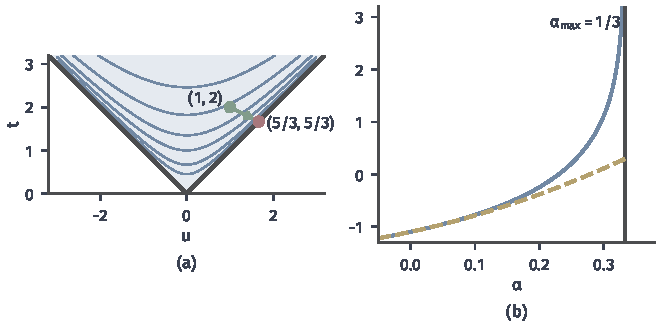
\includegraphics[width=112mm]{figures/05-optimization/06-constrained-optimization/matplotlib/nlipm-soc-barrier/figure.pdf}
  \caption{二阶锥（$q=1$）的障碍。(a)浅蓝区域是锥内部，深灰粗线是锥面，蓝线是$\phi$的等值线。绿点是$(1,2)$，绿色箭头是方向$(2,-1)$，红点是它到达锥面的位置$(5/3,5/3)$。(b)沿该方向的$\phi$（蓝线）与它在$\alpha=0$处的二次模型（黄色虚线），深灰粗线是$\alpha_{\max}=1/3$。}
  \label{fig:nlipm-soc-barrier}
\end{BookInlineFigure}

\paragraph{仿射映射进入锥后的Newton系统}
实际问题的约束通常写成
\[
 \lVert\bm{B}\bm{x}+\bm{e}\rVert_2\leq\bm{a}^\top\bm{x}+d,
\]
也就是$\bm{y}(\bm{x})=\bm{Q}\bm{x}+\bm{q}$落在锥中，这里$\bm{Q}$由$\bm{B}$和$\bm{a}^\top$拼成，$\bm{q}=(\bm{e},d)$。由链式法则，
\begin{equation}
 \nabla_{\bm{x}}\phi=\bm{Q}^\top\nabla\phi(\bm{y}),\qquad
 \nabla_{\bm{x}}^2\phi=\bm{Q}^\top\nabla^2\phi(\bm{y})\bm{Q}.
 \label{eq:nlipm-soc-affine}
\end{equation}

把式~\eqref{eq:nlipm-soc-derivatives}代入，得到的矩阵是“稀疏的$\bm{Q}^\top\bm{R}\bm{Q}$”加上一个秩一矩阵。秩一项的向量$\bm{Q}^\top\bm{R}\bm{y}$通常是稠密的，直接相加会填满矩阵。保留锥结构的实现把它单独存放，或者在鞍点矩阵中增加一行一列，这样既不丢失稀疏性，也能用现成的分解。

\paragraph{展开成标量约束的代价}
也可以把约束写成标量不等式$g(\bm{u},t)=\lVert\bm{u}\rVert_2-t\leq0$，用本章前几节的方法。问题出在$\bm{u}=\bm{0}$：$g$在这里不可微，而这恰恰可能是解所在的位置，例如目标要把$\lVert\bm{B}\bm{x}+\bm{e}\rVert_2$压到零时。图~\ref{fig:nlipm-soc-kink}显示，$-\log(t-\lVert\bm{u}\rVert_2)$在$\bm{u}=\bm{0}$处有折角，$-\log(t^2-\lVert\bm{u}\rVert_2^2)$却是光滑的，因为它用平方把折角消掉了。

改写成$g=\lVert\bm{u}\rVert_2^2-t^2\leq0$并不解决问题。这个$g$不是凸函数，它的零下水平集还包括$t<0$的另一半锥，所以必须同时约束$t\geq0$。二阶锥障碍用$\omega$的同时把定义域限定在$t>0$的内部，避免了这两个麻烦。

\begin{BookInlineFigure}
  \centering
  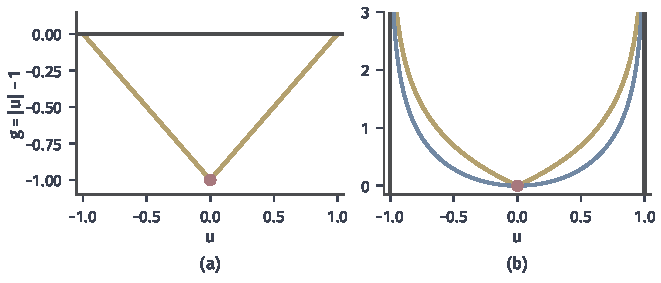
\includegraphics[width=112mm]{figures/05-optimization/06-constrained-optimization/matplotlib/nlipm-soc-kink/figure.pdf}
  \caption{标量写法与锥障碍，$t=1$。(a)标量约束$g=\lvert u\rvert-1$在$u=0$处有折角（红点）。(b)黄线是$-\log(1-\lvert u\rvert)$，保留了折角；蓝线是二阶锥障碍$-\log(1-u^2)$，在$u=0$处光滑。深灰粗线是边界。}
  \label{fig:nlipm-soc-kink}
\end{BookInlineFigure}

\subsection{半正定锥障碍}
\label{sec:nlipm-psd}

变量换成对称矩阵$\bm{X}\in\mathcal{S}^n$，约束是$\bm{X}\succeq\bm{0}$，内积是迹内积
\[
 \langle\bm{X},\bm{Z}\rangle=\operatorname{tr}(\bm{X}\bm{Z}).
\]
半正定锥在这个内积下是自对偶的，所以$\bm{K}^*=\bm{K}$。

\paragraph{特征值逼近零}
$\bm{X}$越靠近边界，最小的特征值越接近零。记$\bm{X}$的特征值为$\rho_1,\ldots,\rho_n>0$，对每个特征值都放一项对数障碍，得到
\begin{equation}
 \phi(\bm{X})=-\sum_{i=1}^n\log\rho_i(\bm{X})=-\log\det\bm{X}.
 \label{eq:nlipm-psd-barrier}
\end{equation}
计算时不必求特征值，$\log\det$可以由Cholesky分解得到。由$\det(\tau\bm{X})=\tau^n\det\bm{X}$，障碍参数是$\vartheta=n$。

\paragraph{线性扰动下的导数}
沿对称方向$\bm{D}$看。因为$\bm{X}\succ\bm{0}$，可以写成
\[
 \bm{X}+\alpha\bm{D}=\bm{X}^{1/2}\bigl(\bm{I}+\alpha\bm{X}^{-1/2}\bm{D}\bm{X}^{-1/2}\bigr)\bm{X}^{1/2}.
\]
记$\bm{X}^{-1/2}\bm{D}\bm{X}^{-1/2}$的特征值为$\beta_1,\ldots,\beta_n$，它们也是$\bm{X}^{-1}\bm{D}$的特征值。取行列式再取对数，得到
\begin{equation}
 \phi(\bm{X}+\alpha\bm{D})=\phi(\bm{X})-\sum_{i=1}^n\log(1+\alpha\beta_i).
 \label{eq:nlipm-psd-expansion}
\end{equation}
对$\alpha$展开到二阶，一阶系数是$-\sum_i\beta_i$，二阶系数是$\sum_i\beta_i^2$。写成迹，就是
\begin{equation}
 \begin{gathered}
 \langle\nabla\phi(\bm{X}),\bm{D}\rangle=-\operatorname{tr}(\bm{X}^{-1}\bm{D}),\\
 \langle\bm{D},\nabla^2\phi(\bm{X})[\bm{D}]\rangle=\operatorname{tr}(\bm{X}^{-1}\bm{D}\bm{X}^{-1}\bm{D}).
 \end{gathered}
 \label{eq:nlipm-psd-derivatives}
\end{equation}
所以在迹内积下$\nabla\phi(\bm{X})=-\bm{X}^{-1}$，Hessian是线性算子$\bm{D}\mapsto\bm{X}^{-1}\bm{D}\bm{X}^{-1}$。

式~\eqref{eq:nlipm-psd-expansion}同时给出最大步长。$\bm{X}+\alpha\bm{D}\succ\bm{0}$当且仅当每个$1+\alpha\beta_i>0$，所以若$\beta_{\min}<0$，
\begin{equation}
 \alpha_{\max}=-\frac{1}{\beta_{\min}},
 \label{eq:nlipm-psd-step}
\end{equation}
否则$\alpha_{\max}=+\infty$。

用具体的矩阵算一遍。取
\[
 \bm{X}=\begin{bmatrix}2&1\\1&2\end{bmatrix},\qquad\bm{D}=\begin{bmatrix}-1&-1\\-1&-2\end{bmatrix}.
\]
$\bm{X}$的特征值是$1$和$3$。直接计算，
\[
 \bm{X}^{-1}\bm{D}=\frac13\begin{bmatrix}-1&0\\-1&-3\end{bmatrix},
\]
它的特征值是$-1/3$和$-1$，所以$\alpha_{\max}=1$。可以核对，$\bm{X}+\bm{D}$的第二行是零，确实落在边界上。

由式~\eqref{eq:nlipm-psd-derivatives}，一阶、二阶导数分别是
\[
 \frac13+1=\frac43,\qquad\frac19+1=\frac{10}{9}.
\]
而$\det(\bm{X}+\alpha\bm{D})=(1-\alpha)(3-\alpha)$，对$-\log$直接求导得到同样的数。图~\ref{fig:nlipm-psd-barrier}显示了特征值沿这个方向的变化和障碍的上升。

\begin{BookInlineFigure}
  \centering
  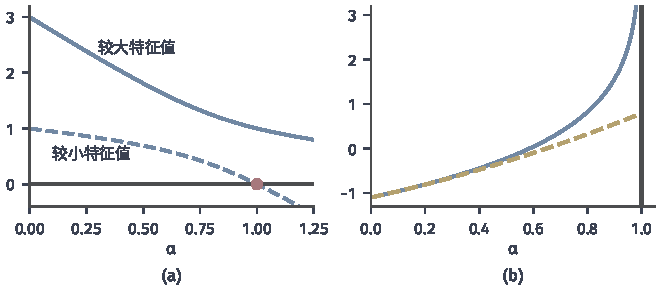
\includegraphics[width=112mm]{figures/05-optimization/06-constrained-optimization/matplotlib/nlipm-psd-barrier/figure.pdf}
  \caption{半正定锥的障碍，沿$\bm{X}+\alpha\bm{D}$。(a)$\bm{X}+\alpha\bm{D}$的两个特征值，红点是较小的特征值到达零的位置$\alpha_{\max}=1$，深灰粗线是零。(b)蓝线是$-\log\det(\bm{X}+\alpha\bm{D})$，黄色虚线是它在$\alpha=0$处的二次模型，深灰粗线是$\alpha_{\max}$。}
  \label{fig:nlipm-psd-barrier}
\end{BookInlineFigure}

\paragraph{矩阵的互补不能照搬标量操作}
中心路径的第三式是$\bm{Z}=\mu\bm{X}^{-1}$，等价于$\bm{X}\bm{Z}=\mu\bm{I}$。标量情形下，线性化$x_is_i=\mu$毫无歧义。矩阵情形下，直接线性化得到
\begin{equation}
 \Delta\bm{X}\,\bm{Z}+\bm{X}\Delta\bm{Z}=\sigma\mu\bm{I}-\bm{X}\bm{Z}.
 \label{eq:nlipm-psd-linearize}
\end{equation}
麻烦在于$\bm{X}$和$\bm{Z}$不交换，$\bm{X}\bm{Z}$一般不对称。解出来的$\Delta\bm{X}$也不对称，走一步之后$\bm{X}$就离开了对称矩阵空间。

看一个具体的例子。取前面的$\bm{X}$，再取$\bm{Z}=\operatorname{diag}(1,2)$，对偶方向$\Delta\bm{Z}$是非对角的对称矩阵。由式~\eqref{eq:nlipm-psd-linearize}解$\Delta\bm{X}$时，出现的项是
\[
 \bm{X}\Delta\bm{Z}\bm{Z}^{-1}=\begin{bmatrix}2&1\\1&2\end{bmatrix}\begin{bmatrix}0&1\\1&0\end{bmatrix}\begin{bmatrix}1&0\\0&1/2\end{bmatrix}=\begin{bmatrix}1&1\\2&1/2\end{bmatrix},
\]
它不是对称的。

解决的办法是\term{原始—对偶缩放}（primal-dual scaling）：选一个可逆矩阵$\bm{P}$，不线性化$\bm{X}\bm{Z}$，而线性化对称化之后的量
\begin{equation}
 \mathcal{H}_{\bm{P}}(\bm{M})=\tfrac12\bigl(\bm{P}\bm{M}\bm{P}^{-1}+(\bm{P}\bm{M}\bm{P}^{-1})^\top\bigr),\qquad
 \mathcal{H}_{\bm{P}}(\bm{X}\bm{Z})=\mu\bm{I}.
 \label{eq:nlipm-psd-scaling}
\end{equation}
三种选择最常见：$\bm{P}=\bm{I}$只把结果对称化；$\bm{P}=\bm{Z}^{1/2}$称为HKM方向；$\bm{P}$取Nesterov—Todd缩放矩阵时，$\bm{X}$与$\bm{Z}$被映到同一个矩阵。不同选择的方向不同，都要保证$\Delta\bm{X}$、$\Delta\bm{Z}$是对称的。

以HKM方向为例，把$\Delta\bm{X}$对称化之后，得到
\[
 \Delta\bm{X}=\sigma\mu\bm{Z}^{-1}-\bm{X}-\tfrac12\bigl(\bm{X}\Delta\bm{Z}\bm{Z}^{-1}+\bm{Z}^{-1}\Delta\bm{Z}\bm{X}\bigr).
\]
代入约束，形成关于$\Delta\bm{y}$的方程，系数矩阵的元素是
\begin{equation}
 M_{ij}=\operatorname{tr}\bigl(\bm{A}_i\bm{X}\bm{A}_j\bm{Z}^{-1}\bigr),
 \label{eq:nlipm-psd-schur}
\end{equation}
其中$\bm{A}_i$是约束$\langle\bm{A}_i,\bm{X}\rangle=b_i$的系数矩阵。它是第~\ref{chap:lp-interior-point}章$\bm{A}\bm{D}\bm{A}^\top$的矩阵版本。

\paragraph{内积配对要保持一致}
实现中常把对称矩阵排成向量，这一步很容易出错。$\bm{X}$有$n(n+1)/2$个独立元素，若直接取上三角排成向量，内积就变了。前面的$\bm{X}$满足$\operatorname{tr}(\bm{X}^2)=10$，而向量$(2,1,2)$的平方和是$9$，因为非对角元在迹里算了两次。

正确的做法是把非对角元乘以$\sqrt{2}$，得到$(2,\sqrt{2},2)$，平方和正好是$10$。对偶变量、梯度和$\mathcal{A}^*$都要用同样的约定，否则对偶可行性和间隙算的都不是原来的量。

\paragraph{三种障碍的对比}
表~\ref{tab:nlipm-barriers}把本章的三种障碍放在一起。形式相同的地方是路径和间隙的公式，不同的地方在互补的写法和步长的求法，这两处决定了线性代数的结构。

\begin{BookInlineTable}
  \centering
  \footnotesize
  \begin{tabular}{@{}llll@{}}
    \toprule
    量 & 标量$s>0$ & 二阶锥 & 半正定锥\\
    \midrule
    障碍 & $-\log s$ & $-\log(t^2-\lVert\bm{u}\rVert_2^2)$ & $-\log\det\bm{X}$\\
    参数$\vartheta$ & $1$ & $2$ & $n$\\
    $-\nabla\phi$ & $1/s$ & $2\bm{R}\bm{x}/\omega$ & $\bm{X}^{-1}$\\
    内积 & 乘法 & 欧氏内积 & 迹内积\\
    $\alpha_{\max}$ & 比值 & 二次方程的根 & $\bm{X}^{-1}\bm{D}$的特征值\\
    线性代数 & 对角 & 对角加秩一 & 稠密缩放矩阵\\
    \bottomrule
  \end{tabular}
  \caption{三种锥的障碍及相应的计算。}
  \label{tab:nlipm-barriers}
\end{BookInlineTable}
